\documentclass{sig-alternate}
\usepackage{graphicx}
\usepackage{amsmath}
\usepackage{amssymb}
\usepackage{natbib}
\usepackage{myAlgorithm}
\usepackage{xcolor}

\bibliographystyle{abbrvnat}

\definecolor{darkred}{rgb}{.5,0,0}

\title{Machine Learning for Predictive Auto-Tuning with Boosted Regression Trees}

% XXX: fix fonts in figures

\numberofauthors{3}

\author{
%\alignauthor First Last\titlenote{}\\
\alignauthor First Last\\
\affaddr{Affiliation line 1}\\
\affaddr{Affiliation line 2}\\
\email{anon@mail.com}
% 2nd author
%\alignauthor First Last\titlenote{None}\\
\alignauthor First Last\\
\affaddr{Affiliation line 1}\\
\affaddr{Affiliation line 2}\\
\email{anon@mail.com}
% 3rd author
%\alignauthor First Last\titlenote{None}\\
\alignauthor First Last\\
\affaddr{Affiliation line 1}\\
\affaddr{Affiliation line 2}\\
\email{anon@mail.com}
}

\begin{document}
\maketitle

\begin{abstract}

% UPDATE ABSTRCT.TXT IF YOU CHANGE THIS!!! (abstract.txt)
Auto-tuning techniques are widely used and effective for optimizing a
parametrized GPU code template for a particular computation on particular
hardware.
However, a drawback of this approach is that thorough or exhaustive
auto-tuning requires compiling many kernels and calling each one many times,
and this process is slow.  Furthermore, it is desirable to provide users
with unified library abstraction boundaries for operations such as image
filtering and matrix multiplication, even those these operations actually
correspond to a large set of potential problem configurations with a wide
variety of memory access patterns and computational bottlenecks.  How can we
draw on data from previous empirical auto-tuning of related problems on related
hardware to make a just-in-time implementation decision for a novel problem?
This paper presents a machine learning approach to auto-tuning, in which
features of the current hardware platform, the kernel configuration and the
problem instance are passed to a regression model (boosted regression trees)
which predicts how much faster this kernel will be than a reference
baseline.  Combinatorial optimization strategies for auto-tuning that would
normally require evaluating large number of kernel configurations on the real
hardware, are made orders of magnitude faster by evaluating the surrogate
regression model instead.  We validate our approach using the filterbank
correlation kernel described in \citet{pinto+cox:2011gcg}, where we find that
0.1 seconds of hill climbing on the regression model (``{\em
predictive} auto-tuning'') can achieve an average of 95\% of the
speed-up brought by minutes of empirical auto-tuning.  Our approach is not
specific to filterbank correlation, nor even to GPU kernel auto-tuning, and can
be applied to almost any templated-code optimization problem, spanning a wide
variety of problem types, kernel types, and platforms.
% UPDATE ABSTRCT.TXT IF YOU CHANGE THIS!!! (abstract.txt)

\end{abstract}

%XXX: use 300\% boost instead of 3x

% %%%%%%%%%%%%%%%%%%%%%%%%%%%%%%%%%%%%%%%%%%%%%%%%%%%%%%%%%%%%%%%%%%%%%%%%%%%%%
\section{Introduction}

% 1 Introduction

% HPC Landscape: from single proc to multi-cores

Due to power consumption and heat dissipation concerns, scientific applications
have shifted from computing platforms where performance had been primarily
driven by rises in the clock frequency of a single ``heavy-weight'' processor
(with complex out-of-order control and cache structures) to a platform with
ever increasing numbers of ``light-weight'' cores. Interestingly, this shift is
now not only relevant to computational sciences but to the development of all
computer systems: from ubiquitous consumer-facing devices (e.g. phones) to
high-end computer farms for web-scale applications (e.g. social networks).

% HPC Landscape: large diversity of architectures,
% no consensus => push to flexibility => push to sw

Although the future lies in low-power multi-core hardware designs, the field
lacks consensus on exactly how the different subsystems (memory,
communication and computation) should be efficiently integrated, modeled and
programmed. These systems have exhibited varying degrees of memory hierarchy
and multi-threading complexity and, as a consequence, they have been
increasingly relying on flexible but low-level software-controlled cache
management and parallelism \citep{asanovic2006landscape} in order to better
control and understand the various trade-offs among performance, reliability,
energy efficiency, production costs, etc. This evolution has profoundly
altered the landscape of application development: programmers are now
facing a wide diversity of low-level architectural issues
that must be carefully balanced if one is to write code that is both
high-performance \emph{and} portable.

% =============================================================================
\subsection{Motivation}

% Better tools: motivation (compilers/tools/libs can’t keep up, it’s too
% difficult)

In this rapidly evolving landscape, the construction of general
development tools and libraries that fully utilize system resources
remains a daunting task. Even within specialized architectures from the
\emph{same} vendor, such as NVIDIA's Graphics Processing Units (GPUs) and the
Compute Unified Device Architecture (CUDA) \citep{nickolls2008scalable,
nvidia2011cuda}, many developers default to massive amounts of manual labor
to optimize CUDA code to specific input domains. In addition, hand-tuning
rarely generalizes well to new hardware generations or different input
domains, and it can also be error-prone or far from optimal. One of the
reason is that kernels can produce staggeringly large optimization spaces
\citep{datta2008stencil}. The problem is further compounded by the fact that
these spaces can be highly discontinuous \citep{ryoo2008program}, difficult
to explore, and quasi-optimal solutions lie at the edge of ``performance
cliffs'' induced by hard device-specific constraints (e.g. register file
size or low-latency cache size).

% =============================================================================
\subsection{Auto-Tuning}
% Related Work instead ??
% XXX: a reference to brewer1995high

% auto-tuning is an answer

One strategy for addressing these challenges is to use one of a variety of
automatic methods known collectively as ``auto-tuning.'' Two major auto-tuning
approaches have emerged in the extensive literature covering the subject (see
surveys in
\citep{vuduc2001statistical, demmel2005self, vuduc2005oski, williams2008auto,
datta2008stencil, cavazos2008intelligent, li2009note, park2011evaluation}):
analytical model-driven optimization and empirical optimization
\citep{yotov2003comparison}.

% model-driven optimization: intro

The model-driven optimization approach uses analytical abstractions to model
the hardware architectures, in order to identify possible code transformations and their complex
interactions. Even though highly-accurate analytical models are generally
difficult to build, this approach has been quite successful in the past, especially for 
accelerating serial code, utilizing simplified but general abstractions. However,
large speed-ups for parallel code require more accurate high-dimensional models
and since this approach is bound by the quality and scalability of its
abstraction, it has been less suited for highly-specialized kernels. This
approach has been well-developed in the compiler community, and as a result, it has
most often been applied at compile-time where important run-time characteristics
such as input domains may be missing. These limitations render the model-driven
optimization approach less attractive in many high-performance library development settings.

% * empirical optimization: intro / advantages

The empirical optimization approach, in contrast, seeks to find the best
performing code configuration by automatically generating many versions of a
parametrized kernel and benchmarking them on the actual hardware (possibly at
runtime, when contextual information about the hardware and software stack is
the richest). This method directly optimizes the metric(s) of interest (e.g. performance) and does not rely on
surrogates.  A significant advantage of such approaches is that they allow any metric to be
optimized without loss of generality. Indeed, it is possible to formulate a multi-objective optimization that minimize both run time \emph{and}
power consumption \citep{rahman2011automated}, a feat that would be even more difficult using an
analytical model-driven approach. Due to its flexibility,
empirical auto-tuning has been successfully applied to build a variety of high-performance
domain-specific libraries including dense linear algebra
\citep{clint2001automated, bilmes1997optimizing}, sparse linear algebra
\citep{vuduc2005oski}, signal processing \citep{frigo2005design}, sorting
\citep{li2004dynamically}, general stencil operations \citep{kamil2010auto}, etc.

% empirical optimization: disadvantages

The empirical approach is very sensitive to the choice of instrumented
optimizations \emph{and} to the search method. The size of the search space is
often so large that the current best empirical auto-tuners typically only consider
highly-specialized functions with a limited set of code transformations and
compiler options, on a limited set of input domains \citep{ganapathi2009case}. Although
searches for good code configurations in highly-discontinuous spaces can
be made ``embarrassingly'' parallel, and thus benefit from parallel execution across many devices, it remains a prohibitively
expensive combinatorial optimization problem, as many variants of the code must
generated, compiled, and benchmarked on specific input domains with meaningful
statistics (that may require multiple runs). Consequently, most proposed
methods prune the space with hard-coded heuristics that offer little
generalization guarantees. This has been a key drawback of the empirical
approach as compared to the model-driven approach, where good code configurations
can be directly derived from the analytical model.

% hybrid optimization: the bad way

To ameliorate this weakness, it is intuitively appealing to combine the two
approaches by first constraining the search space with an analytical model and
then exploring the reduced space empirically \citep{chen2005combining,
li2009note}. Unfortunately, such a hybrid approach is still bound by the quality
of the analytical model, which remains hard to build by hand.

% hybrid optimization: the ML way (note that ML-based are in essence
% model-driven too just with an empirically learned model)

In this paper, we propose to \emph{learn the model} using non-linear regression
modeling techniques instead of constructing a model manually. By learning the model, one can
hope to achieve elements of the best of both approaches: the search speed of model-based auto-tuning with the broad applicability
and ease of implementation of empirical auto-tuning.

Various statistical prediction techniques have been applied with
success at compile-time for general programs on various CPU architectures
\citep{monsifrot2002machine, stephenson2003meta, yotov2003comparison,
kulkarni2004fast, cooper2005acme, franke2005probabilistic,
hutter2006performance, cavazos2007rapidly, cavazos2008intelligent,
hartono2009annotation, park2011evaluation, fursin2008milepost}.
Relative to this work, our contribution is to show
how to do fast predictive auto-tuning that satisfies the requirements to:
(a) handle the variety of recent multi-core architectures like GPUs \citep{schaa2009exploring},
(b) provide high-performance domain-specific libraries \citep{nukada2009auto, li2009note, kamil2010auto},
(c) that select good implementations at run-time \citep{klockner2011pycuda, pinto+cox:2011gcg}, and
(d) for the full input domain of a library routine \citep{liu2009cross, grauer2011optimizing}.
% XXX: are these last references appropriate
% XXX: there are 4 versions of the stencil work - consolidate to just the full journal version


The paper is organized as follows:
Section~\ref{sec:brtree} describes the boosted regression tree model and the procedure for fitting it to empirical timing data.
Section~\ref{sec:kernel} describes the sort of kernel we employ for our benchmarking,
Section~\ref{sec:exp} presents the results of our benchmarking experiments, which
compare a reference implementation to a) empirical auto-tuning over a domain-specific grid,
b) empirical auto-tuning over a hill-climbing search, and
c) predictive auto-tuning.
%Section~\ref{sec:discussion}.
Section~\ref{sec:previous} summarizes previous and related work involving  machine learning with performance auto-tuning.
Section~\ref{sec:conclusion} summarizes our findings and outlines directions for future work.

% %%%%%%%%%%%%%%%%%%%%%%%%%%%%%%%%%%%%%%%%%%%%%%%%%%%%%%%%%%%%%%%%%%%%%%%%%%%%%
\section{Predictive Auto-Tuning}

\begin{figure}[!ht]
\centerline{
\begin{algorithm}{$\Algo{\color{darkred}{autotune\_empirical}}\big(shapes, strides \big)$}
\Aitem $a \setto TaskFeatures(shapes, strides)$
\Aitem $c \setto PlatformFeatures()$
\Aitem $b^* \setto \operatorname*{argmin}_{b \in \mathcal{B}} MeasureTime(a, b, c)$
\algoremark{\color{darkred}{slow}}
\Aitem \Return $b^*$
\end{algorithm}
}
\begin{algorithm}{$\Algo{\color{darkred}{autotune\_predictive}}\big(shapes, strides \big)$}
\Aitem $a \setto TaskFeatures(shapes, strides)$
\Aitem $c \setto PlatformFeatures()$
\Aitem $f \setto TimingModel()$
\Aitem $b^* \setto \operatorname*{argmin}_{b \in \mathcal{B}} f(a, b, c)$
\algoremark{\color{darkred}{fast}}
\Aitem \Return $b^*$
\end{algorithm}
\caption{Pseudo-code template for empirical and predictive auto-tuning.
Empirical auto-tuning (above) is inevitably slow
because dynamically-generated code must be compiled and run on a number of actual-size inputs.
Predictive auto-tuning (below) can be orders of magnitude faster. We show that it can
also be accurate.
}
\label{fig:general_autotune}
\end{figure}

This work shows that auto-tuning can be accelerated by orders of
magnitude by using a regression model built offline as a surrogate for actual
computations on the real hardware.
The general form of an auto-tuning based library routine is illustrated in Figure~\ref{fig:general_autotune} (top).
An auto-tuning based routine must operate on three sets of variables:
\begin{description}
\item[$\mathcal{A}$:] task description (argument shapes, physical layout)
\item[$\mathcal{B}$:] implementation description (auto-tuning parameters)
\item[$\mathcal{C}$:] platform description (capabilities, micro-benchmarks)
\end{description}
The hypothetical auto-tuning routine described at the top of Figure~\ref{fig:general_autotune}
might take many minutes or hours to perform the argmin at step 3 (during which time it computes the desired result many times!)
so it would not be suitable for a normal library subroutine implementation.
However, the form of the auto-tuning routine suggests the potential for enormous acceleration:
if only there were a fast (even approximate) surrogate for the costly $MeasureTime(\cdot)$ function,
then the argmin could be done in a fraction of a second and the routine could be used normally (Figure~\ref{fig:general_autotune}, bottom).

\subsection{Learning a Regression Model}

The heart of predictive auto-tuning is a regression model that acts as surrogate
for a hand-crafted hardware model or empirical timing estimates.
In our experiments, this regression model fits empirically measured timing information for a {\em subset} of the configuration space and interpolates / extrapolates that timing across the remainder of the space.
To fit this model, we
form a training set $\mathcal{X}, \mathcal{Y}$ where
each point $x^{(i)} \in \mathcal{X}$ is a tuple $(a^{(i)}, b^{(i)}, c^{(i)})$
and each target $y^{(i)} \in \mathcal{Y}$  reflects the speed of implementation $b^{(i)}$
on inputs $a^{(i)}$ on platform $c^{(i)}$.

The effectiveness of predictive auto-tuning depends on the mapping between the raw kernel timings $t(a, b, c)$ (i.e. in seconds) and the utility $y$ associated with that timing.
Anticipating that regression involves minimizing the squared error of our predictor (see Eq.~\ref{eq:y}) it is important to choose $y$ so that differences of a given numerical {\em magnitude} correspond to {\em improvements} of a certain utility.
In program optimization we are interested in improving the speedup over a reference implementation $b^{(\mathrm{ref})}$, so it is natural to choose
\begin{equation}
y^{(i)}
= \log\left(\frac{\mathrm{speed}(a, b, c)}{\mathrm{speed}(a, b^{(\mathrm{ref})}, c)} \right)
= \log\left(\frac{t(a, b^{(\mathrm{ref})}, c)}{t(a, b, c)} \right)
\label{eq:y}
\end{equation}

One unique aspect of our setting compared with standard regression
is that not all kernel implementations ($b$) are {\em valid}
for all input configurations. One option for dealing with these invalid configurations
would be to simply omit them from $\mathcal{X}$ and $\mathcal{Y}$, but that would lead to a biased regression model.
Instead, we chose to associate invalid $(a, b, c)$ tuples with a constant $y = \zeta$.
It makes sense to choose $\zeta < 0$ so that invalid configurations are treated as being worse than the reference,
but the question of how much worse these points should be is an empirical one.
Our experiments evaluate $\log(0.01) \leq \zeta \leq \log(.99)$.

% =============================================================================
\subsection{Regression Trees}
\label{sec:brtree}

A regression tree is a piece-wise constant function from one vector space to another,
that works by recursively subdividing the input space into constant regions~\citep{breiman+friedman+olshen+stone:1984, hastie+tibshirani+friedman:2001}.
They are widely used in statistics and data-mining applications because the fitting algorithm is quick and reliable, and the form of the tree can provide insight into the relevant input variables.
We use a standard fitting procedure, which takes a set of
$(x, y)\in \mathbb{R}^k \times \mathbb{R}$ pairs and constructs a tree with a low mean squared error.
To construct each node of a regression tree,
we sort the set $\mathcal{D}$ of ($x,y$) pairs along each of the $k$ features to find the best partitioning $f_{i,\gamma}$ of the input space along feature $i$ at point $\gamma$ (Eqs.~\ref{eq:figamma}, \ref{eq:treeloss}).
\begin{align}
    f_{i,\gamma}(x) &=
    \begin{cases}
        \alpha  &\text{if $x_i < \gamma$} \\
        \beta &\text{if $x_i \geq \gamma$}
    \end{cases}
    \label{eq:figamma}\\
    i^*, \gamma^* &= \operatorname*{argmin}_{i, \gamma} \mathbb{\hat E}\left[ (y - f_{i,\gamma}(x))^2 \right]
    \label{eq:treeloss}
\end{align}
One disadvantage of the regression tree is that it does not make full use of broad patterns in the data -- each partition formed by the fitting procedure is fit independently in the recursive training procedure,
so it impossible for the model to extract more than one bit of information from each training partition.
% XXX unclear
This disadvantage is mitigated to a significant extent by the practice of {\em boosting}.

% =============================================================================
\subsection{Boosted Regression Trees}

Boosting is an iterative procedure for constructing an {\em ensemble} of regression trees that is coordinated to fit training examples as accurately as possible.
\citep{schapire:2001,friedman:2002}
In a recent empirical study of a range of machine learning regression problems,
boosted decision trees were found to be among the best and easiest models to
apply~\citep{caruana+niculescu-mizil:2006}.
On each boosting iteration, a regression tree is fit to the residual error remaining
after all previously-fit models have made their predictions.
There are essentially three parameters that control the boosted regression tree
training procedure:
1) the depth of tree constructed on each boosting iteration,
2) the minimum number of examples to allow at a regression tree leaf, and
3) the number of trees constructed by boosting.
We did not attempt a systematic study of the effect of these variables on performance.
We chose a maximum depth of 4,
a minimum number of examples of 10,
and 100 iterations of boosting.

\subsection{Search Algorithms}

Once an accurate regression model has been fit to the data, it remains to be optimized for novel arguments (Fig.~\ref{fig:autotune_general}, bottom, step 4).
An exhaustive search is the most reliable if it can be afforded, but in our experiments
(as in general) an exhaustive search is prohibitively expensive.
In our experiments we compare two strategies:
(1)
a generic stochastic hill-climbing search,
and (2)
a hand-chosen grid provided by the authors of the kernel used in our experiments \citep{pinto+cox:2011gcg}.
The {\em hill-climbing} (HC) search algorithm starts from the reference
implementation and resamples each of the parameters
of the current best implementation randomly with
probability $0.25$ (keeping the current best setting with probability $0.75$).
On each hill-climbing iteration, if the speed of the newly sampled point is greater than the previous point, then it becomes the current point.
We show results for search variants HC25, HC50, and HC75, which correspond do hill-climbing for 25, 50, and 75 iterations respectively.
The {\em grid} algorithm is specific to the kernel used in our case study,
the details of the grid are provided with our experimental results in Section~\ref{sec:refgrid}

% %%%%%%%%%%%%%%%%%%%%%%%%%%%%%%%%%%%%%%%%%%%%%%%%%%%%%%%%%%%%%%%%%%%%%%%%%%%%%
\section{Filterbank Correlation}

\label{sec:fbcorr}

Filterbank correlation is a simple spatial image filtering operation that is
an important subroutine in many image processing applications. It has a relatively
high arithmetic intensity which makes it a natural fit for GPU platforms~\citep{pinto+cox:2011gcg}.

Mathematically, we define filterbank correlation in terms of an
image $x$ and a filterbank $f$.
The image $x$ has $R$ rows, $C$ columns, and $D$ channels (e.g. color
channels) that we call its {\em depth}. We index $x$ like $\mathbf{x}[i,j,d]$
where $0 \leq i < R$, $0 \leq j < C$, and $0 \leq d < D$.
The filterbank $f$ has $F$ filters that are like little images: each has a
height $H$, a width $W$, and $D$ channels.
We will restrict ourselves to what are called {\em valid} correlations, in
which the image is larger in both rows and columns than the filters.
The result of filterbank correlation of $x$ with $f$ is an image-like array
$z$ with $R-H+1$ rows, $C-W+1$ columns, and depth $F$, whose elements are
defined according to Equation~\ref{eq:z}:

\begin{equation}
    \mathbf{z}[r,c,k] = \sum_{w=0}^{W-1} \sum_{h=0}^{H-1} \sum_{d=0}^{D-1}
        \mathbf{x}[r+h, c+h, d]~ \mathbf{f}[k, h, w, d].
        \label{eq:z}
\end{equation}

In terms of floating point operations, a filterbank correlation requires the
inner sums to be computed for each output pixel, yielding the quantity in
Eq.~\ref{eq:flops}:
\begin{equation}
\mathrm{FLOPS} = 2  F  H  W  D  (R - H + 1)( C- W + 1)
\label{eq:flops}
\end{equation}
The multiplicative factor of 2 arises because we must first multiply an element of
$x$ with an element of $f$ and then add the result to an element of $z$.

The memory transfer requirements of filterbank correlation are more difficult to quantify.
Assuming three kinds of non-register memory -- constant, shared, and global --
and assuming optimistically that the entire filterbank fits into the GPU's constant memory,
then we can establish a lower bound (Eq.~\ref{eq:bytes}) on the amount of
memory that must be moved in order to store the computed result to global
memory starting from arguments in global memory:
\begin{align}
\mathrm{Bytes} = 4&RCD \nonumber \\
& + 4FHWD \nonumber \\
& + 4(R-H+1)(C-W+1)F.
\label{eq:bytes}
\end{align}
In short, we must read the filterbank and image once, and store the result.

The arithmetic intensity of filterbank correlation, assuming our lower bound on memory transfers
is therefore approximately
\begin{align}
\mathrm{intensity} & \approx \frac {FDHW} {2(D+F)},
\end{align}
for images that are large relative to filters.
Each $F$ output writes corresponds to approximately $D$ input reads
and $F$ inner products between $DHW$ elements.

The high potential for arithmetic intensity makes the GPU an ideal platform for computing filterbank correlations,
and and filterbank correlation is used extensively in image and video processing,
where it is often a computational bottleneck.
One might expect then, that it would be easy to implement a library providing
this operation as a simple function that takes pointers and strides for $x$, $f$, and $z$ and performs the computation.
However, as shown in \citet{pinto+cox:2011gcg} 
it is challenging to provide an implementation
or even an implementation strategy that provides satisfactory performance
across the range of inputs (shapes, physical layouts) that occur in
typical usage.
\citet{kamil+etal:2009} summarize a related situation related to general stencil computations in their abstract:
``Although the auto-tuning strategy has been successfully applied to libraries,
generalized stencil kernels are not amenable to packaging as libraries.''



% %%%%%%%%%%%%%%%%%%%%%%%%%%%%%%%%%%%%%%%%%%%%%%%%%%%%%%%%%%%%%%%%%%%%%%%%%%%%%
\section{GPU Implementation}
\label{sec:kernel}

The strategy we use for computing filterbank correlation on the GPU
using CUDA follows \citet{pinto+cox:2011gcg}.
The overall strategy is to load the filterbank into constant memory, which is
relatively fast and visible to all threads, and then launch a grid of blocks
that tiles the output image.
Each thread computes $4 \times n\_output\_4s$ channels for some column and row of $z$.
Each block of threads computes $4 \times n\_output\_4s$ channels for a sub-rectangle of the output image ($z$).
When there are more than $4 \times n\_output\_4s$ channels in $z$, or if the
filterbank is too large to fit into constant memory, then multiple
kernel executions perform the full computation.
Our approach permits splitting the filterbank along
the number-of-filters dimension ($F$) and the height dimension ($H$).
All the filterbanks in our study are small enough that
at least one row of a single filter can fit into constant memory.
Pseudo-code for the kernel is given in Figure~\ref{fig:kernel}.

\begin{figure}[!ht]
\centerline{
\begin{algorithm}{$\Algo{thread\_fbcorr}\big(gX, cF, gZ \big)$}
\Aitem shared $sX \setto$ all channels of region ($\beta$) of $gX$
\Aitem $x, y \setto$ position of this thread in output image
\Aitem \_\_syncthreads()
\Aitem $v[0:N] \setto 0$, for $N=4\times n\_output\_4s$
\Aitem for $d \setto 0$~\To~$D$,
\Aitem ~ for $h \setto 0$~\To~$H / n\_filter\_r$,
\Aitem ~ ~ for $w \setto 0$~\To~$W$,
\Aitem ~ ~ ~ $u \setto sX[x+h, y+w, d]$
\Aitem ~ ~ ~ for $n \setto 0$~\To~$n\_output\_4s - 1$,
\Aitem ~ ~ ~ ~  $v[n] \setto v[n] + cF[n, h, w, d]$
\Aitem for $n \setto 0$~\To~$n\_output\_4s - 1$,
\Aitem ~  gZ[x][y][4n:4n+n] += v[4n:4n+n], (float4)
\end{algorithm}
}
\caption{Kernel pseudo-code for filterbank correlation.
Input $gX$ is a pointer to $x$ in global memory, input $cF$ is a pointer to
$f$ in either constant or texture memory, and output $gZ$ is a pointer to $z$
in global memory.
Each block of threads modifies $4 \times n\_output\_4s$ channels of a
rectangle (called $\beta$ in code listing) within $z$. A grid of blocks covers all rows and columns of $z$.
Multiple calls can be used to apply all filters of a large filterbank $f$ to
$x$.
}
\label{fig:kernel}
\end{figure}

The kernel is parametrized by 10 parameters:
\begin{align*}
\mathrm{block\_h}    & \in (4, 8, 16, 32, 64, 128) \\
\mathrm{block\_w}    & \in (4, 8, 16, 32, 64, 128) \\
\mathrm{n\_filter\_r} & \in (1, 2) \\
\mathrm{n\_output\_4s} & \in (\mathrm{all}, 1, 2) \\
\mathrm{spill}      & \in (False, True) \\
\mathrm{imul\_fast}  & \in (False, True) \\
\mathrm{pad\_shared} & \in (False, True) \\
\mathrm{use\_tex1d}  & \in (False, True) \\
\mathrm{maxrreg}    & \in (8, 16, 20, 24, 28, 32, \infty) \\
\mathrm{fast\_math}  & \in (False, True)
\end{align*}

The block height (``block\_h'') and block width (``block\_w'') parameters control the
number of threads that run within each block.
Each kernel call loads some number of filter rows (``n\_filter\_r'') into
constant memory and processes the correlation of the image with just those
rows, incrementing the output buffer.
Each thread can compute several output elements
at once, in multiples (``n\_output\_4s'') of 4;
this increases the efficiency of each thread, but can lead to lower occupancy.
Registers are a precious commodity on the GPU, and this kernel accumulates
elements of $v$ in registers.
The ``spill'' parameter controls whether the current thread's output position in
$gZ$ is stored in a register (faster access) or in shared memory (frees up
a register).
The ``imul\_fast'' parameter controls whether integer multiplication is done
in 24-bit (True) or 32-bit (False) precision.
The ``pad\_shared'' parameter controls whether the $sX$ shared memory buffer
is padded, which wastes space in shared memory but reduces bank conflicts.
The ``use\_tex1d'' parameter controls whether the image is loaded into shared
memory with global pointer dereferences or texture fetches.
The ``maxrreg'' and ``fast\_math'' parameters are passed to the nvcc compiler to limit
the number of registers available to each thread, and to enable more aggressive instruction selection, respectively.


When the entire filterbank does not fit into the GPU's
constant memory, $P$ passes are necessary to compute all of $z$, where
$$P=\frac{FH}{4 \cdot n\_output\_4s \cdot n\_filter\_r}.$$
In such cases, the number of bytes moved to and from global memory is much higher than
the theoretical lower limit.
\begin{align}
\mathrm{Bytes} = 4&RCDP \nonumber \\
& + 4FHWD \nonumber \\
& + 8(R-H+1)(C-W+1)FP.
\nonumber
\label{eq:bytesP}
\end{align}
These passes make the I/O requirements increase quadratically in $F$ and $H$.
At the same time, the total number of floating-point operations (Eq.~\ref{eq:flops})
is quadratic in $H$ and $W$. In our experiments, we only considered square
filters so in our setting the total number of flops is proportional to $H^4$.

Critically:
what makes this kernel interesting as a case study is that the
arithmetic intensity, shared storage, and register requirements
of this kernel change significantly and in a complicated platform-dependent way
with the argument parameters ($R, C, D, F, H, W$) and with the implementation parameters,
especially ``block\_w'', ``block\_h'', ``n\_output\_4s'' and ``n\_filter\_rows.''


\subsection{Reference and Grid}
\label{sec:refgrid}

\cite{pinto+cox:2011gcg} recommends as a reference implementation: block\_w 8, 
block\_h = 8, n\_filter\_rows 1, n\_output\_4s all, spill $False$, imul\_fast $True$,
pad\_shared $True$, 
use\_text1d $True$,
maxrreg $\infty$,
and fast\_math $False$.
This reference implementation was chosen manually based on good performance across a range of platforms from older-generation
cards such as the
8600GT all the way to
current-generation flagship cards such as the GTX 580 and C2070.
Given that parameters were hand-chosen for the reference kernel, no claims are
made as to the optimality nor universality of this reference (indeed, different
programmers would undoubtedly arrive at different results).  We use this
kernel configuration as a reasonable indicator of typical performance
made possible by ad hoc experimentation with parameters.

Additionally, \cite{pinto+cox:2011gcg} advocate a particular grid search over
what was estimated to be the most relevant part of the configuration space.
This grid iterates over all
combinations of n\_filter\_rows, n\_output\_4s, spill\_l, pad\_shared\_l for three different block\_h, block\_w choices: (16, 8), (16, 16), and (32, 8).
In our experiments, we call this algorithm the {\em grid} search procedure.
The grid included $72$ points in addition to the reference implementation, for a total of $73$ points.

\subsection{Software Stack}

This kernel was implemented in the meta-programming style advocated in
\citet{pinto+cox:2011gcg} in Python using Cheetah for string
processing~\citep{cheetah} and PyCUDA~\citep{klockner2011pycuda} for dynamic
kernel compilation and interfacing with CUDA.

% %%%%%%%%%%%%%%%%%%%%%%%%%%%%%%%%%%%%%%%%%%%%%%%%%%%%%%%%%%%%%%%%%%%%%%%%%%%%%

\section{Experimental Setup}

Recall from the introduction (Eq.~\ref{eq:condopt}) that auto-tuning can be seen
as a conditional optimization problem in which we seek an implementation ($b \in \mathcal{B}$) that minimizes runtime or some other scalar-valued cost function
for given arguments ($a \in \mathcal{A}$) on a particular platform ($c \in \mathcal{C}$).
In order to perform predictive auto-tuning with a regression model,
it is necessary to characterize these
three types of variables with {\em features}.
%In Section~\ref{sec:modeling} we see how these features are used as inputs to
%the regression model in predictive auto-tuning.
We describe the arguments to a filterbank correlation with the 6-tuple
$(R, C, D, F, H, W)$.
We randomly sampled arguments (uniformly) from the following product space:
\begin{align*}
R = C & \in \{ 256, 512, 1024, 2048, 4096 \} \\
H = W & \in \{ 3, 5, 7, 9, 11 \} \\
D &  \in \{1, 4, 8, 16, 32, 64, 128, 256 \} \\
F &  \in \{1, 4, 8, 16, 32, 64, 128, 256 \}
\end{align*}

A library implementation of this operation would ideally support all image and
filter sizes as well as variations due
to strided memory layouts. In such a setting it would be useful to characterize
the arguments with
features such as whether the inputs are Fortran-style contiguous, C-style contiguous, or row-padded to various byte alignments.
These additional options would make our
approach of automatic auto-tuning even more important, because there would be
a greater variety in the kinds of computations and memory transfers to
perform.
Our experiments consider a somewhat simplified setting in which the arguments are always stored
with depth channels being contiguous in memory, followed by columns, then rows, and then filters having the largest stride.

The product space in our study
includes 1600 argument combinations, but we restricted our experiments to correlations that
represented between 1 and 50 gigaflops of arithmetic.
Smaller problems do not fully utilize GPU hardware and are handled equally well by many kernel settings.
Larger take so long to evaluate that there is negligible
inefficiency in implementing them via multiple calls with smaller images and fewer filters.
With the experiments searched an argument space included 602 configurations with between 1 and 50 gigaflops.

For the implementation features $b$, we directly used the integer and binary
values (block\_w, block\_h, etc.) that parametrized the kernels.  We did not
use platform features ($c$) in our experiments. We leave the investigation of
cross-platform predictive auto-tuning for future work.

% %%%%%%%%%%%%%%%%%%%%%%%%%%%%%%%%%%%%%%%%%%%%%%%%%%%%%%%%%%%%%%%%%%%%%%%%%%%%%
\section{Results}

\begin{figure*}[!t]
\centering
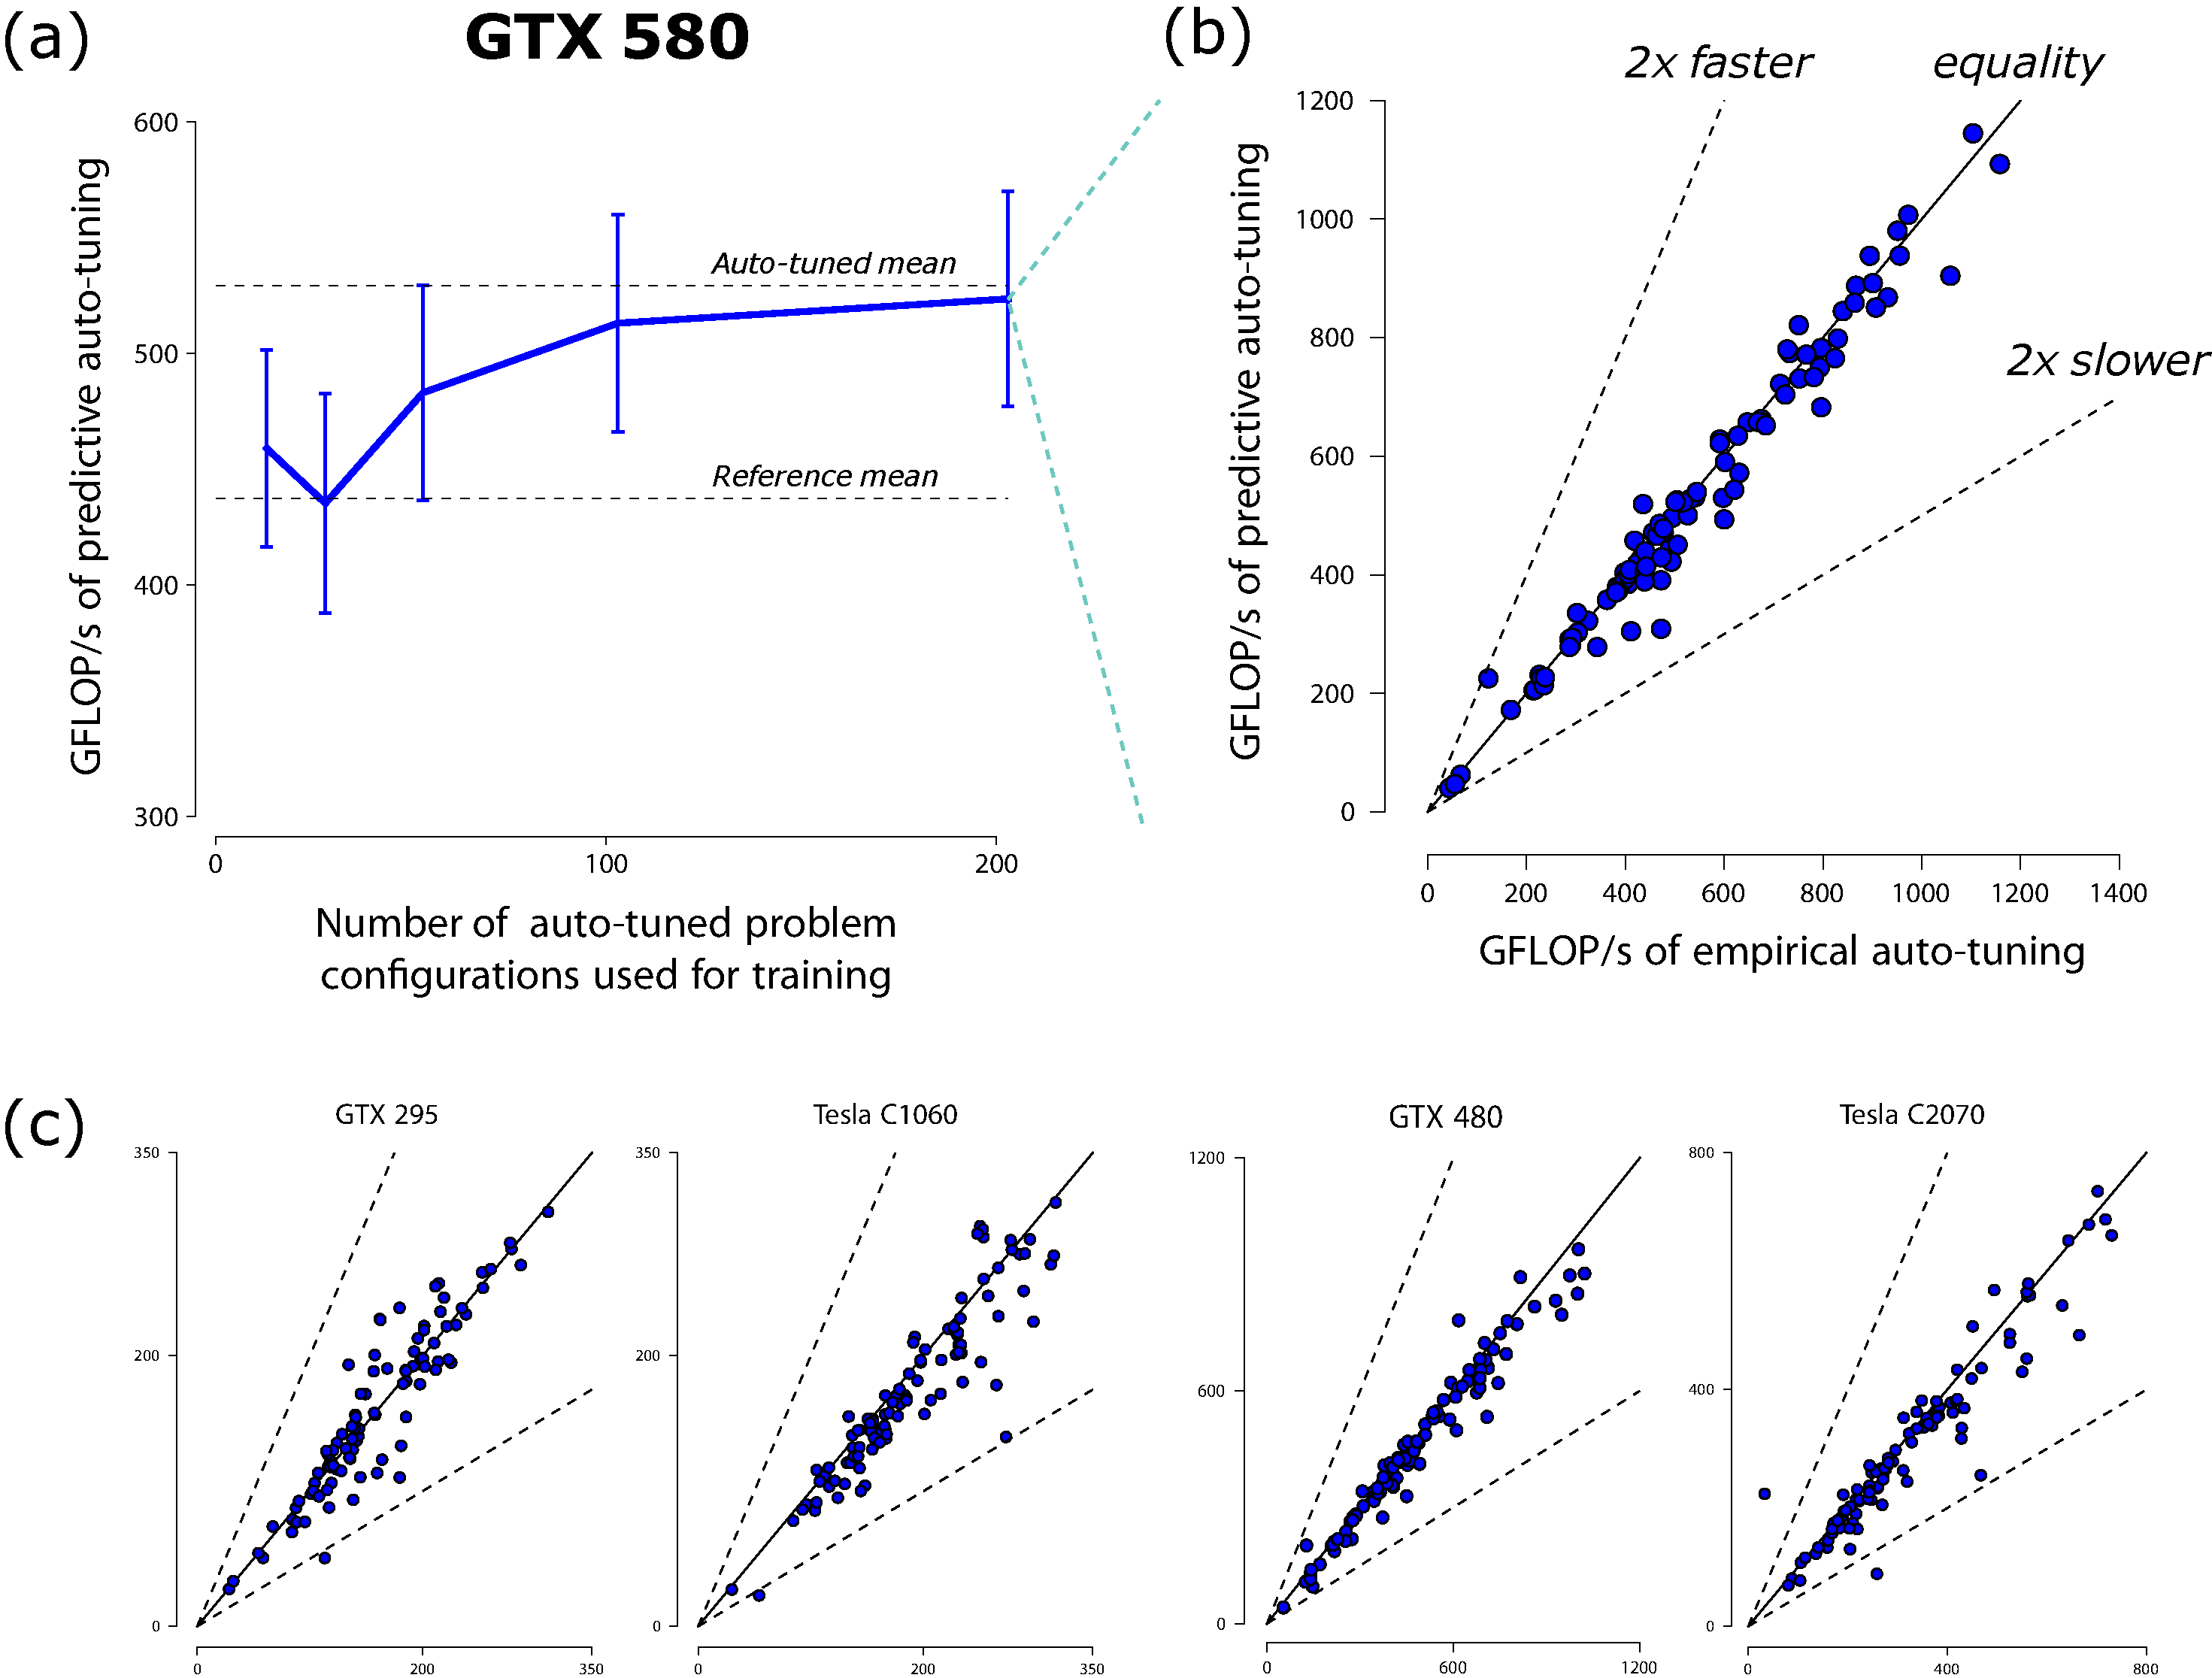
\includegraphics[width=.9\linewidth]{illustrator/fig_main_R1.pdf}
\caption{
Computation speed for novel problem configurations using predictive
vs. empirical auto-tuning.
(a) As more problem configurations are used to train the regression model,
the performance of predictive auto-tuning approaches that of empirical auto-tuning
despite taking only 0.1 seconds instead of 2 minutes.
(b) and (c) For a wide range of devices, implementation speeds found by predictive auto-tuning correlate tightly with
implementation speeds found by empirical auto-tuning.
%The boosted regression trees used for predictive auto-tuning generalize correctly across the implementation space.
}
\label{fig:fig_gflop_scatter}
\end{figure*}


Figure~\ref{fig:allstars} shows the effectiveness of empirical auto-tuning is
in this setting.  Taking the GTX 295 as an example, and averaging across the
range of problem configurations in our study, we find that empirically
auto-tuned implementations are on average about 50\% faster than the reference
implementation.  The reference in turn, is about 50\% faster than
implementations that were empirically auto-tuned for a \emph{randomly chosen}
different argument configuration.  This shows that it is genereally not enough
to auto-tune for particular argument configurations; instead it is important to
choose the right kernel for the job for each unique argument configuration
(input-dependent auto-tuning).

Comparing the {\em grid} to {\em HC25}, {\em HC50} and {\em HC75} we found very
little difference in performance.  The HC25 was slightly poorer, but the grid,
HC50, and HC75 algorithms delivered similar average results. None of the
algorithms was strictly better than the others.  In our predictive
auto-tuning experiments we used HC75.

% formation of training set

Figure~\ref{fig:fig_gflop_scatter} shows how accurate predictive auto-tuning is compared with empirical auto-tuning.
The training set $(\mathcal{X}, \mathcal{Y})$ for the regression model comprised
all of the $<(a,b,c), y>$ pairs observed during grid search and hill-climbing search.
So for each training argument configuration $a,c$ there were 148 different values of $b$ and thus 148 training points.
Figure~\ref{fig:fig_gflop_scatter} (a) shows that as more argument configurations are used for training,
the performance of predictive auto-tuning on test configurations $(a', c)$ quickly
approaches the average performance of empirical auto-tuning.
We took care to partition the train and test sets so that there were no overlapping configurations.
The key difference between the predictive and empirical auto-tuning,
is that predictive auto-tuning
typically took about 0.1 seconds per test example, whereas empirical auto-tuning took about 1-3 minutes.

Figure~\ref{fig:fig_gflop_scatter} (b) and (c) show that the implementation
speeds found by predictive auto-tuning correlates very well with the speed of
empirical auto-tuning across all of the devices we tested: GTX 580, GTX 480,
GTX 295, Tesla C2070, and Tesla C1060 which span three generations of
CUDA platforms.

% backtracking
In some cases, predictive auto-tuning yields an invalid implementation.  We
dealt with this scenario by backtracking through the various best-estimates
discovered during the hill-climbing search.  Some invalid kernels can only be
discovered after compiling code and attempting to run the compiled code, so in
these cases predictive auto-tuning took up to 3 seconds.  Even in these cases
the predictive model is much faster than empirical auto-tuning, because the
first kernel that actually runs is a fast one.

Figure~\ref{fig:fig_ntrain} shows how the training set size
and the value of $\zeta$ affect the accuracy of predictive auto-tuning.
All candidates timed during the grid and
hill-climbing search procedures were used as training examples, so the training
set sizes ranged from an average of 1480 (10 problem configurations) to 29 600
(200 problem configurations).
Training from the largest training sets took approximately 30 seconds.
Training 50 or more problem configurations yielded quite accurate predictions
with $\zeta=\log(0.5)$, which was the best value for $\zeta$ across the range of
devices in our study.

\begin{figure}[!t]
\centering
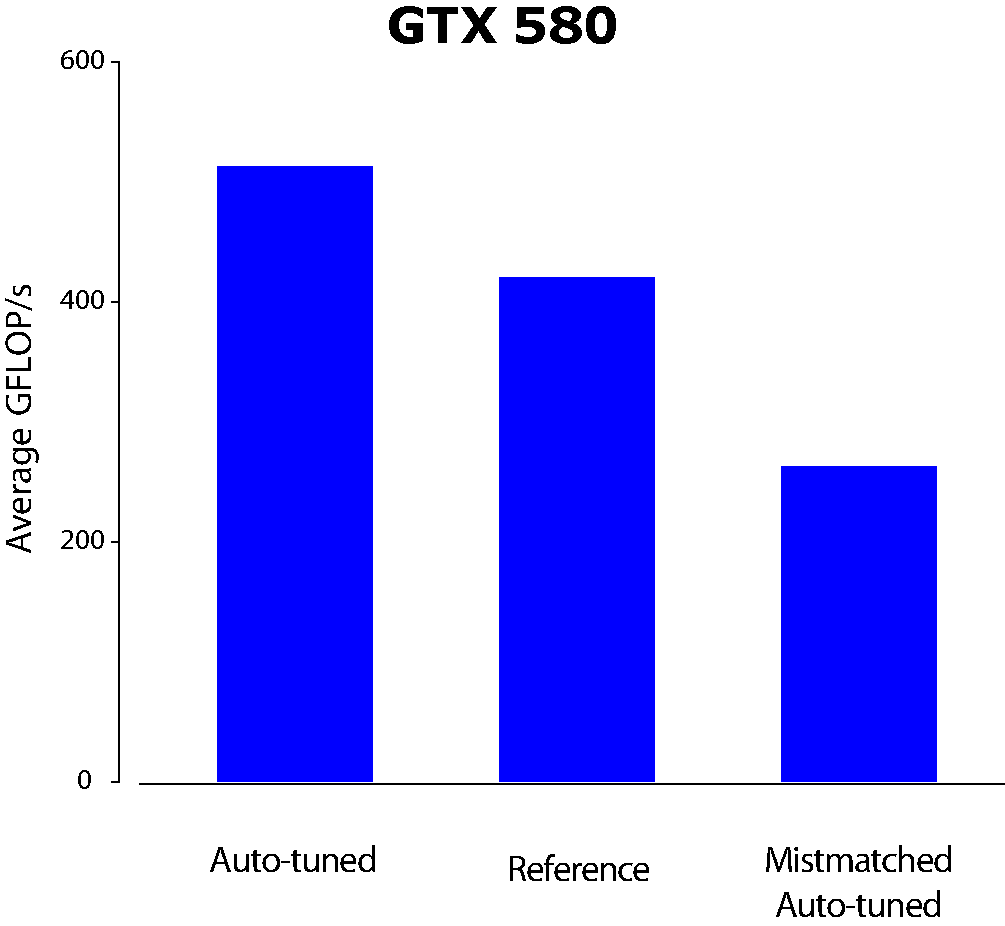
\includegraphics[width=\linewidth]{illustrator/fig_allstars_mixup_580_R1.pdf}
\caption{Different arguments call for different kernels:
{\em left} is the average argument-specific empirical
auto-tuned performance across 100 random argument configurations,
{\em middle} is the average speed of our reference implementation,
{\em right} is the average speed of kernels auto-tuned for different argument
configurations than the one being tested.  For 38/100 random configurations, the
kernel auto-tuned for another problem could not even run on the GTX 295
hardware.  These points contributed a speed of 0, bringing down the average
much lower than the reference.  Good performance across a variety of inputs
requires {\em input-dependent auto-tuning}.
}
\label{fig:allstars}
\end{figure}

\begin{figure}[!t]
\centering
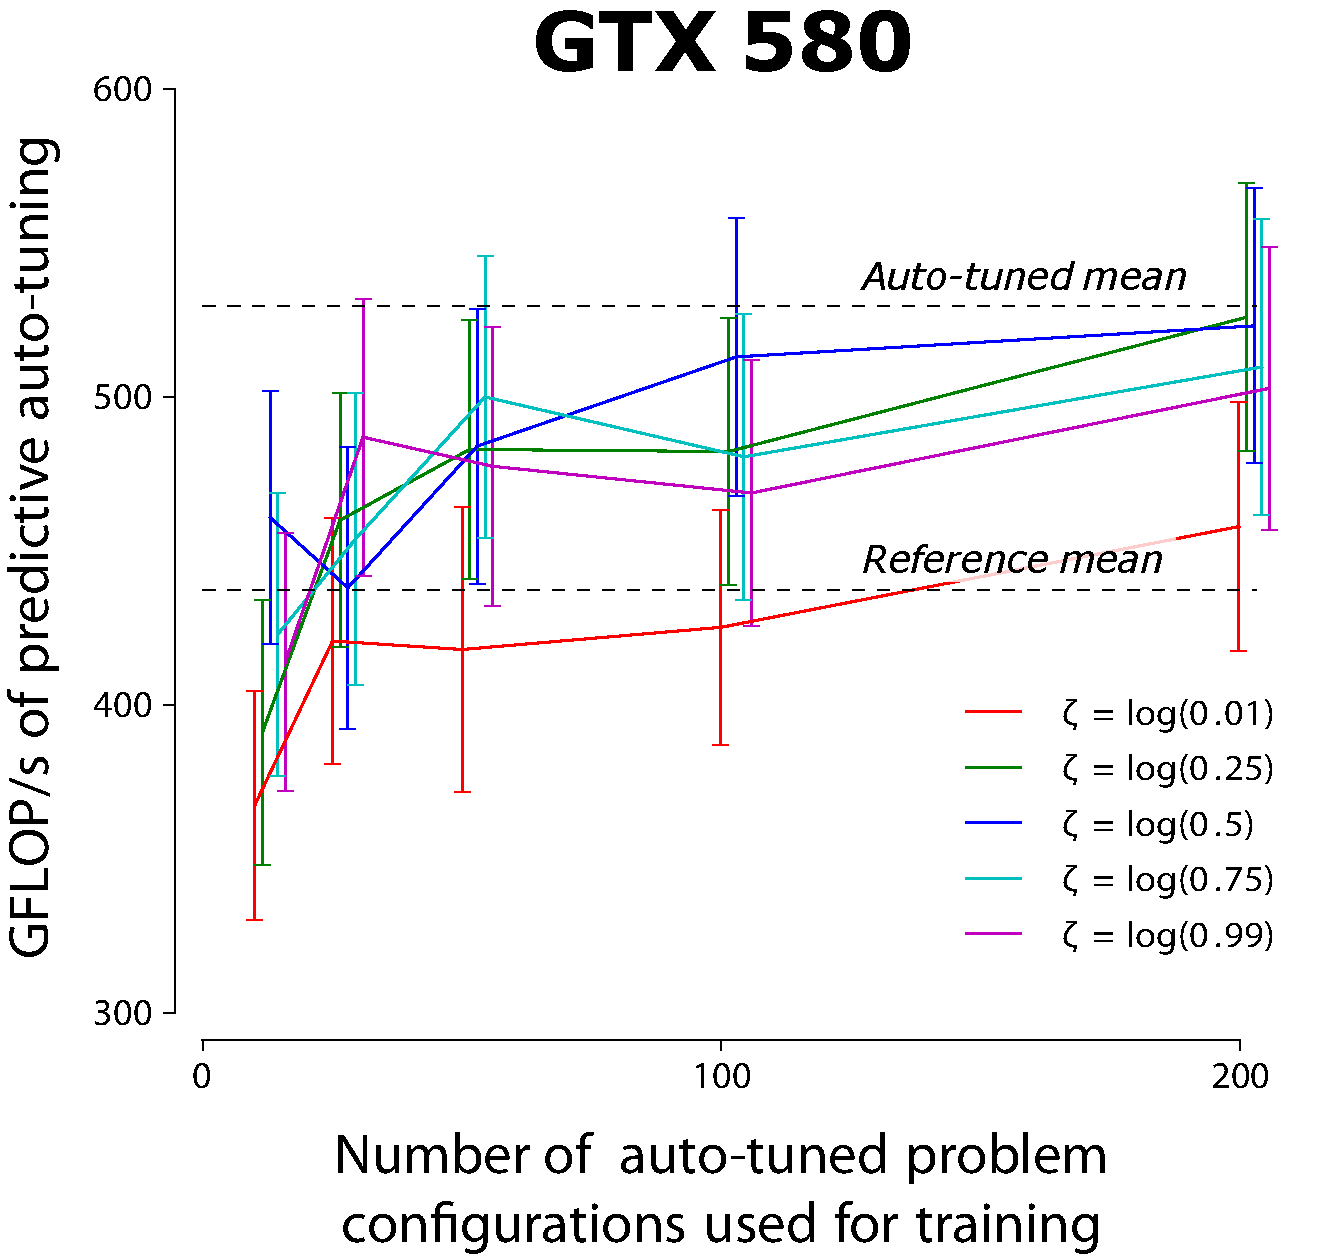
\includegraphics[width=\linewidth]{illustrator/fig_ntrain_munctional0_580.pdf} % on vader
\caption{The effect of the invalid configuration score ($\zeta$) and training set
size on predictive auto-tuning.
Models trained on as few as 25 configurations outperformed the reference.
Models trained on 50 or more configurations rivaled empirical auto-tuning.
Moderate values of $\zeta$ between $\log(0.25)$ and $\log(0.75)$ are best.
}
\label{fig:fig_ntrain}
\end{figure}


% %%%%%%%%%%%%%%%%%%%%%%%%%%%%%%%%%%%%%%%%%%%%%%%%%%%%%%%%%%%%%%%%%%%%%%%%%%%%%
\section{Discussion}

% say what we said
In this paper, we've demonstrated a boosted regression tree-based auto-tuning
method, wherein empirical performance data is used to train a machine learning
model of performance for an instrumented GPU kernel.  In contrast to
traditional model-based auto-tuning, where an explicit model of performance is
built on the basis of an understanding of hardware inner workings, and
empirical auto-tuning, where an exhaustive set of implementation configurations
are tried, the present approach generates, from scratch, a model of kernel
performance on the basis of timing data from a user-definable number of kernel
evaluations.  This approach allows significant flexibility to navigate
trade-offs between offline and run-time costs, and final auto-tuning
performance.  Importantly, this method treats kernels as black-boxes, allowing
the user to auto-tune in the absence of deep knowledge of hardware details
(which may even been unknowable, in the case of hardware not available at the
time of kernel creation).  This approach also frees auto-tuning performance
from a strong dependency on the accuracy (or inaccuracy) of a pre-defined
analytical model.

An important use case for the tools described here is in the development of
user-facing numerical libraries.  Such libraries are a critical component of
scientific computing infrastructure, since they abstract away implementation
details and make algorithms available to a much wider audience.  However, the
abstraction provided by libraries represents a double-edged sword: one hand,
\emph{using} the library is easier, because it presents a unified abstraction
of related functionality.  However, at the same time, any given library routine
might represent a wide range of substantially different problem configurations,
each with distinct computational issues and bottlenecks.  Auto-tuning has long
provided a solution that finesses these two issues, providing multiple
implementations under the hood, for multiple problem settings, and then using
heuristics or explicit, hand-crafted models to select the appropriate
implementation for a given set of inputs.  The development of such auto-tuned
libraries, while extremely successful, is also very difficult.  The
machine-learning-based techniques described here provide a middle ground, where
a library developer can simply create an instrumented kernel, and allow
generic tools to automatically generate appropriate auto-tuned implementations,
with small (and controllable) run-time costs.

% DDC: the following text looks like random dumping ground

% We're characterizing hardware by a 1-of-N feature vector, simply describing
% which hardware is the current hardware.
% To make better use of auto-tuning data from other platforms, it would be more
% useful to have precise and descriptive features such as: what compute
% capability is present, how many cores are active, what is the bandwidth
% between the various kinds of memory, and how much of various kinds of memory
% is present.  With these features a model-assisted auto-tuning approach
% might be able to make very good guesses on hardware for which no auto-tuning
% has ever been done.
% 
% In a complete implementation of Eq.~\ref{eq:z}, there would be parameters
% related to the physical layout (e.g. strides) of $x$, $f$ and $z$ arrays in
% addition to the mathematical parameters of heights and widths and so on,
% so the total number of filterbank correlation computations that a user might
% be able to demand is astronomical.
% A typical coping mechanism would be to cast an arbitrary problem configuration into a more
% standardized form, such as by copying inputs into aligned memory buffers with
% appropriate padding, and then choosing an appropriate blocking strategy for
% the computation. At that point, auto-tuning efforts can be focussed on the
% kernel for each blocked strategy. However, on GPU hardware, the cost of
% aligning the inputs can be relatively large.  In future work we hope to apply
% our model-based technique to auto-tune in full problem configuration space, so
% that we can optimize as much of the computation as possible within the
% predictive auto-tuning framework (XXX name).
% 
% Platform Space: XXX
% 
% %\renewcommand{\bibsection}{\section*{Bibliography}}
% %\setlength{\bibsep}{5pt}
% 
% 
% 
% One might expect then, that it would be easy to implement a library providing
% this operation -- this hypothetical library could have quite a simple interface
% following the spirit of FFTW or a BLAS routine:
% \begin{verbatim}
%     gpu_fbcorr(
%         img_shape, filters_shape,
%         img, filters, output)
% \end{verbatim}
% However, as shown in \citet{pinto+cox:2011gcg} and numerous articles on
% related stencil operations XXX, it is challenging to provide an implementation
% or even an implementation strategy that provides satisfactory performance
% across the range of inputs (shapes, physical layouts) that occur even in
% typical usage.
% 
% Current state-of-the art is to do empirical auto-tuning.
% XXX \vspace{12pt}
% 
% Increasingly, machine learning and statistical inference strategies are
% finding application in compiler technology.
% XXX \vspace{12pt}
% 
% machine learning
% 
% This paper shows that a kernel with several  boosted
% 
% 
% There is a natural function from
% problem space x implementation space x platform space to runtime:
% how much wall time elapses on the given platform when solving the given
% problem with the given implementation.
% 
% Auto-tuning is a family of empirical techniques for finding the implementation
% that minimizes that runtime function, when the platform and the problem
% configuration are given.
% 
% XXX: some math, or possibly a picture with the three boxes that was on Pinto's
% whiteboard.
% 
% This paper is about different ways of doing the minimization.
% For a particular problem (filterbank correlation) we
% look at a parameterized kernel implementation (from \citet{pinto+cox:2011gcg})
% and a few hardware platforms, and compare
% random search, grid search, and a hill-climbing strategy with a good, but
% generic, reference implementation.
% Then we show that we can model the LSM function with a regression tree
% well enough to usefully perform the argmin of Equation~\ref{eq:lsm_argmin}
% on the model rather than the actual system. Whereas it may take several
% minutes to perform a hill-climbing or grid search in the original system,
% a hill-climbing search in the model requires a small fraction of a second.
% Model-based auto-tuning makes it possible to simulate auto-tuning quickly and
% accurately enough to be used within a single library call of the computational
% routine.
% 
% Best arithmetic density
% 
% A bandwidth analysis that takes the blocking structure into account would
% reveal that larger $H$ and $W$ require each block to read a larger input
% region, and store it in a larger shared memory region, which reduces the
% potential for high occupancy.
% 
% Filterbank correlation represents a difficult code-optimization problem
% because of the number of interacting constraints: a large value of $P$ reduces
% arithmetic density, but a small value of $P$ requires that each thread do more
% work, and makes global memory access latency harder to hide. (XXX: is there a
% better reason?)
% 
% 
% The kernel used to perform
% filterbank correlation was parametrized by 10 parameters, some of which
% were binary and others of which were integer-valued. The full configuration
% space included 12000 kernels.
% XXX: how to make sense of these paramters without code listing?
% 
% XXX: What to all the parameters mean?
% 
% XXX: how many configurations are in the configuration space
% 
% XXX: what was the reference kernel, and how was it chosen?
% 
% XXX: analysis of READ traffic, WRITE traffic, DATA re-use and CACHEing
% strategies. FLOPS per write etc.
% 
% XXX: Why not use FFT: convolution in spectral domain?
% 
% XXXX: Talk about memory transfer requirements vs. speed vs. copy...
% 
% we believe that our approach is the most practial one to get high perf on
% recent hardware, since there is no consensus on hw features (and it won't
% change soon)
% 
% XXX: deliver significant performance increases at very low run-time cost (less
% than a second if the input domain has not been seen before, zero if it
% has, since it will hit the cache) compared with the reference
% implementation
% 
% XXX always delivered good performance: optimality without loss of productivity?
% 
% XXX such machine learning derived model-based empirical auto-tuner hold great
% promise for dev productivity, portability, performance on future multi-core hw
% with different architectural features
% 
% XXX frameworks for predicting performance exist \cite{XXX Hwu An Adaptive
% Performance Modeling Tool for GPU Architectures}
% but for non-GPU architectures
% 
% auto-tuning required hardward expertise *and* application-domain knowledge, we
% want to remove these restrictions ultimately we want a ml-based approach to
% code optimization that will where a set of generic but deep code
% transformations, could be templated and injected in any domain-specific
% library. this will reduce the need for specialized expertise across the range
% of targeted computing systems.

% %%%%%%%%%%%%%%%%%%%%%%%%%%%%%%%%%%%%%%%%%%%%%%%%%%%%%%%%%%%%%%%%%%%%%%%%%%%%%
\section{Future Work}

While the present work serves as a basic demonstration of the value of using
machine learning models to predict optimal implementation parameters, there are
many avenues for taking these ideas further. A natural route to extend of our
current approach is to include more features as inputs to the predictive model.
In addition to further instrumentation of the kernel in question, input
features could include a much broader range of hardware-related information,
from more detailed information about device capabilities to micro-benchmarks
\citep{wong2010demystifying}, and results from performance limiter analyses
\citep{micikevicius2010analysis}. Such additional features would increase the
predictive model's ability to adapt to a wide range of different kinds of
hardware, including new devices not available at the time of kernel creation.

Another potentially interesting avenue of research is in interpreting the model
learned by predictive auto-tuning.  While traditional model-based auto-tuning
approaches by design assume a given model, and empirical auto-tuning approaches
are completely model free, the predictive approach described here
\emph{generates} a model from performance data.  Because this generated model
can be interrogated by a variety of means, a significant opportunity exists to
learn about the factors that drive the performance of a given kernel.  These
insights can be used to further guide the development and instrumentation of
the kernel, potentially yielding even greater gains.

% more features (this is the hardest, and most manual part, may require
% domain-specific knowledge, but not necessariyly, e.g. microbenchmarking)
% * features derived from micro-benchmarking \citep{wong2010demystifying}
% * features derived from performance limiter analysis \citep{micikevicius2010analysis}

% DDC: these aren't terribly general / interesting to a broad audience

% * more instrumentation
% * more data-layout
% * more threading strategies to lower latency
% (finding a good representation is key, again...)
% 
% online distributed auto-tuning with learning, especially w/ HT-based
% experiments \cite{HT} our method is indeed very well suited for parallel
% explorating of multiple configurations for learning (in a cluster, e.g. in HT
% context) this may get us \emph{more} than linear speed ups for better accuracy,
% especially when more features will be present (see above)
% 
% interpret the learned model and confront the performance against theoreticial
% (or approximated) models of mem/com/compute, arithmetic intensity, etc. to
% understand performance limiters, the hardware, etc.

% DDC: XXX is "Conclusion" a "required" section in any sense.  If not, I think we could probably do without
%\section{Conclusion}

%Our 

{\small
    \bibliography{local}
}
\end{document}

% FOR Extra material see scratch.tex
